\subsection{An algorithm for $\appSVP$ on a $q$-ary lattice} \label{subsec:qAryAlg}

In this section, we present a combinatorial algorithm that on input $\AMat \in \Z_q^{n \times 2n}$ and $\cg < \cq/2 - 1/2$, outputs a vector $\vvec \in \qLATTp(A) \subset \Z_q^{2n}$ s.t.\ $\| \vvec \| \leq n^{\cg+\cq/2+1/2}$. Notice that we set the lattice dimension $m$ as $m=2n$. This choice simplifies the exposition and is necessary for the improved algorithm described in Sect.~\ref{subsec:qAryAlgImproved}. Case $m=\cm n$ for $\cm = \TLandau(1)$ is considered in Rmk.~\ref{rmk:Linm}.%We make such a choice of $m$ for two reasons. First, it simplifies the description of the algorithms and, second, another constant will not make our algorithm faster. 

The algorithm is actually a combinatorial \BKW-type algorithm for \LWE due to Kirchner-Fouque \cite{C:KirFou15} and Guo et al.\ \cite{C:GuoJohSta15} adapted to the $\appSVP$ problem. We now give its high-level overview.

The idea is to split the dimension of the lattice, $2n$, into $k$ blocks $d_1, \ldots, d_k$, i.e.\ $\sum_{i=1}^k d_i = 2n$. We also choose $k$  positive values $R_1, \ldots, R_k$ where $R_i < q/2$ for all $i$. The algorithm proceeds in $k$ steps. 

On Step 1, we search for pairs of lattice-vectors $(\vvec_1, \vvec_2)$ s.t.\
\[
\Big\lfloor \frac{[\vvec_1]_1^{d_1}}{R_1} \Big\rceil =  \Big\lfloor \frac{[\vvec_2]_1^{d_1}}{R_1} \Big\rceil\footnote{Recall the notation $[\xvec]_i^j = x_i\ldots x_j$ for $i \leq j$.}.
\]
In other words, we split our $q$-ary cube $[-\frac{q-1}{2}, \frac{q-1}{2}]^{d_1}$ (assume $q$ is odd, the algorithm can be easily adapted for an even $q$) into many smaller cubes $[-R_1, R_1]^{d_1}$ and search for pairs $(\vvec_1, \vvec_2)$ that on their first $d_1$ coordinates lie in the same cube. In our algorithm we set $R_1 = n^{\smallo(1)} \ll q $, and we can adjust our choice for $R_1$ s.t. the small cubes split the large cube evenly. See Fig.~\ref{fig:Bucketing} for a $2$-dimensional example. 

Once two such vectors are found, we subtract one from the other and put the result into list $L_1$. Important is that we can bound the $\ell_{\infty}$-norm of elements in $L_1$: on average, $\| [\vvec_1 - \vvec_2]_1^{\d_1}\|_{\infty} \leq \sqrt{2}R_1$. The output of Step 1 are many vectors with \emph{bounded} $\ell_{\infty}$-norm on their first $d_1$ coordinates. On Step 2, we use vectors from $L_1$ to search for pairs that lie in the same $[-R_2, R_2]^{\d_2}$ cube on their $d_1+1, \ldots, d_2$ coordinates analogously to Step 1. The output of Step 2 is a list $L_2$ with vectors bounded in $\ell_{\infty}$-norm on coordinates $1, \ldots, d_1$ and $d_1+1, \ldots, d_2$.  

Repeating this procedure for all $k$ steps, we end up with lattice-vectors for which we can bound their $\ell_{\infty}$-norm on all the $2n$ coordinates and hence, their Euclidean norm. From the upper-bound on the length of the output, we find an optimal on $k$. We defer the discussion on how to set $R_i$'s and $k$ to the next section. 

\begin{figure}[t]
	\centering
	\begin{tikzpicture}
	\draw[gray!20, ->] (-90pt,0) -- (90pt,0);
	\draw[gray!20, ->] (0,-80pt) -- (0,80pt);
	
	 \draw[thick] (-60pt, -60pt) rectangle (60pt, 60pt);
	 \draw (-60pt, 0)  node[below left] {\scriptsize $-\tfrac{q-1}{2}$};
	 \draw (60pt, 0)  node[below right] {\scriptsize $\tfrac{q-1}{2}$};
	 
	 \draw[very thin] (-20pt, -60pt) -- (-20pt, 60pt);
	 \draw[very thin] (20pt, -60pt) -- (20pt, 60pt);
	 \draw[very thin] (-60pt, -20pt) -- (60pt, -20pt);
	 \draw[very thin] (-60pt, 20pt) -- (60pt, 20pt);
	 
	 \draw [decoration={brace, mirror, raise=7pt},
	 		decorate,below=10pt, yshift=5pt](-20pt, 0) -- (20pt, 0) node [black,midway, yshift=-8pt] {\scriptsize $R$};
	 		
	 \filldraw (45pt, 45pt) circle (1pt) node[below right, xshift=-3pt, yshift=2pt] {\tiny $\vvec_1$};
	 \filldraw (32pt, 35pt) circle (1pt) node[below left, xshift=6pt, yshift=2pt] {\tiny $\vvec_2$};
	 
	 \draw [decoration={brace, raise=5pt},
	 	 		decorate,above=10pt, yshift=-3pt, xshift=2pt](32pt, 35pt) -- (45pt, 45pt) node [black,midway, rotate=37, yshift=5pt, xshift=-4pt] {\tiny $ \leq \mkern-6mu \sqrt{2}R$};
	 	 		
	%----------LABELS---------
	\node[draw=none] at (10pt, -15pt){\tiny $(0,0)$};
	\node[draw=none] at (10pt, 25pt){\tiny $(0,1)$};	
	\node[draw=none] at (10pt, -55pt){\tiny $(0,-1)$};
	
	\node[draw=none] at (50pt, 25pt){\tiny $(1,1)$};
	\node[draw=none] at (50pt, -15pt){\tiny $(1,0)$};
	\node[draw=none] at (50pt, -55pt){\tiny $(1,-1)$};
	
	\node[draw=none] at (-30pt, 25pt){\tiny $(1,-1)$};
	\node[draw=none] at (-30pt, -15pt){\tiny $(-1,0)$};
	\node[draw=none] at (-33pt, -55pt){\tiny $(-1,-1)$};
	\end{tikzpicture}
	\caption[Bucketing on a $2$-dimensional $q$-ary lattice]{Bucketing on a $2$-dimensional $q$-ary lattice. Each small cube of length $R$ gets its two-dimensional label. The vectors $\vvec_1$, $\vvec_2$ appear in the same bucket $(1, 1)$ and, hence, the $\ell_2$-norm of their difference is bounded by $\sqrt{2}R$.}
	\label{fig:Bucketing}
\end{figure}

There is one simple trick which greatly improves the running time of the algorithm. We can write our input matrix $\AMat \in \Z_q^{n \times 2n}$ as $\AMat = [\AMat_1 | \AMat_2]$ where $\AMat_i \in \Z_q^{n \times n}$. With high probability, we have that $\AMat_1$ is invertible $\bmod~q$ allowing us to write $\AMat = [\Id_n | \AMat']$ where $\AMat' = \AMat_1^{-1} \AMat_2 \bmod q$. Essentially this procedure brings a $q$-ary code generated by $\AMat$ to a systematic form. It is easy to verify that a basis for $\qLATTp(\AMat)$ is of the form (cf. with the basis $B$ for $\qLat(\AMat\transpose)$ given in Eq.~(\ref{eq:LWEBasis})):
\begin{equation}\label{eq:BasisD}
	\DMat = \begin{pmatrix}
	-\AMat' & q\Id_n \\
	\Id_{n} & 0
	\end{pmatrix}.
\end{equation}


\begin{algorithm}[t]
	\caption{$\appSVP$ on a $q$-ary lattice}
	\label{alg:ApproxSVP}
	\textbf{Input:} $D$ -- a basis for the lattice $\qLATTp(A) \subset \Z_q^{2n}$ defined as in Eq.~(\ref{eq:BasisD}), $\gamma = n^{\cg}$ -- the approximation factor, $\cg>0$ \\
	\textbf{Output:} $L_k$ -- list of vectors from $\qLATTp(A)$ with vectors of norm $\| \vvec \| \leq n^{\cg+\cq/2+1/2}$;
	
	\begin{algorithmic}[1]
		
		\State Set the sieving bounds $R_i$ as $R_1 = n^{\smallo(1)}$ and $R_i = \sqrt{2}^{i-1} R_1$ for $i \geq 2$.
		\State Set the lengths of blocks $d_i$ as in Eq.~(\ref{eq:d_i}) and the boundaries of each block $(l_{i-1}, \ldots, l_i)$ s.t.\ $l_{i}-{l_{i-1}} = d_i$ and $l_k = 1, l_0 = n$.
		
		\Repeat \Comment{Create the list $L_0$}
		\State Choose $\xvec \in \Z_q^{2n}$ s.t.\ $\| [\xvec]_{n+1}^{2n} \|_{\infty} \leq R_1$
		\State $L_0 \gets L_0 \union \{D\xvec \bmod q\} $
		\Until{$L_0$ is large enough}
		
		\State $T \gets \emptyset$ \Comment{Initialize an array $T$ indexed by buckets}
		\ForAll {$i=1 \ldots k$} \label{algline:ForLoop1}
			\ForAll { $\vvec \in L_{i-1}$} \label{algline:ForLoop2}
				\State $b \gets \Big\lfloor \frac{[\vvec]_{l_i}^{l_{i-1}}}{R_i} \Big\rceil$ \Comment Find the bucket for $\vvec\mkern2mu[l_i, \ldots, l_{i-1}]$
				\If{$T[b] = \emptyset$}
					\State $T[b] \gets \vvec$
				\Else
					\State $L_{i} \gets L_{i} \union \{T[b] - \vvec \}$
					\State $T[b] \gets \emptyset$
				\EndIf
			\EndFor
		\EndFor
		\State \Return $L_k$
	\end{algorithmic}
	
	\vspace{10pt}
	
\end{algorithm}

\begin{figure}[H]
	\centering
	\begin{tikzpicture}[]
	\tikzset{
		List/.style={
			rectangle split, rectangle split horizontal,  
			draw=black, thick,
			%text width=10em,
			inner sep=6pt,
		} 
	}    
	\matrix (m) [row sep=0.8em, column sep=3em]{
		\node[](L0) {$L_0:$}; & 
		\node[List, rectangle split parts=3, name=list, rectangle split part fill={black!60,black!60,black!10}] (list) {
			\nodepart[text width=5.4cm]{one}{}
			\nodepart[text width=0.6cm]{two}
			\nodepart[text width=6cm] {three}};
		
		\draw [decoration={brace, raise=5pt},
		decorate,below=10pt] (list.two split north) -- (list.north east) node [black,midway, yshift=20pt] {\scriptsize $n$}; 
		
		\draw [decoration={brace,raise=5pt},
		decorate,below=10pt](list.one split north) -- (list.two split north) node [black,midway, yshift=20pt] {\scriptsize $d_1$};
		
		\draw [decoration={brace, mirror, raise=5pt},
		decorate,below=10pt](list.two split south) -- (list.south east) node [black,midway, yshift=-10pt] {\scriptsize $\leq R_1$};
		
		\draw [decoration={brace, mirror, raise=5pt},
		decorate,below=10pt](list.south west) -- (list.two split south) node [black,midway, yshift=-10pt] {\scriptsize $\leq q/2$};
		\draw [decoration={brace,raise=18pt},
		decorate,below=10pt](list.north west) -- (list.north east) node [black,midway,yshift=30pt] {\scriptsize $2n$};\\[-1ex]
		%---------------------------------------  
		\node[](L1) {$L_1:$}; & 
		\node[List, rectangle split parts=4, name=list2, rectangle split part fill={black!60,black!60,black!15,black!15}] (list2) {
			\nodepart[text width=4.2cm]{one}{}
			\nodepart[text width=0.8cm]{two}
			\nodepart[text width=0.6cm] {three}
			\nodepart[text width=6cm] {four}};
		
		\draw [decoration={brace,raise=5pt},
		decorate,below=10pt](list2.three split north) -- (list2.north east) node [black,midway, yshift=20pt] {\scriptsize $n$}; 
		
		\draw [decoration={brace,raise=5pt},
		decorate,below=10pt](list2.two split north) -- (list2.three split north) node [black,midway, yshift=20pt] {\scriptsize $d_1$};
				
				
		\draw [decoration={brace, mirror, raise=5pt},
		decorate,below=10pt](list2.two split south) -- (list2.south east) node [black,midway, yshift=-10pt] {\scriptsize $\leq \sqrt{2}R_1$};

		
		\draw [decoration={brace,raise=5pt},
		decorate,below=10pt](list2.one split north) -- (list2.two split north) node [black,midway, yshift=20pt] {\scriptsize $d_2$};
		
		\draw [decoration={brace, mirror, raise=5pt},
		decorate,below=10pt](list2.south west) -- (list2.two split south) node [black,midway, yshift=-10pt] {\scriptsize $\leq q/2$};\\ [-1ex]
		
		%---------------------------------------  
		\node[](L2) {$L_2:$}; & 
		\node[List, rectangle split parts=5, name=list3, rectangle split part fill={black!60,black!60,black!30,black!30,black!30}] (list3) {
					\nodepart[text width=3.0cm]{one}{}
					\nodepart[text width=0.8cm]{two}
					\nodepart[text width=0.8cm]{three}
					\nodepart[text width=0.6cm] {four}
					\nodepart[text width=6cm] {five}};
				
		\draw [decoration={brace,raise=5pt},
		decorate,below=10pt](list3.four split north) -- (list3.north east) node [black,midway, yshift=20pt] {\scriptsize $n$}; 
				
		\draw [decoration={brace,raise=5pt},
		decorate,below=10pt](list2.two split north) -- (list2.three split north) node [black,midway, yshift=20pt] {\scriptsize $d_1$};
								
		\draw [decoration={brace, mirror, raise=5pt},
		decorate,below=10pt](list3.three split south) -- (list3.south east) node [black,midway, yshift=-10pt] {\scriptsize $\leq 2 R_1$};
		
		\draw [decoration={brace,raise=5pt},
		decorate,below=10pt](list3.two split north) -- (list3.three split north) node [black,midway, yshift=20pt] {\scriptsize $d_2$};
				
		\draw [decoration={brace, mirror, raise=5pt},
		decorate,below=10pt](list3.two split south) -- (list3.three split south) node [black,midway, yshift=-10pt] {\scriptsize $\leq  \mk \sqrt{2}R_2$};
		
		\draw [decoration={brace,raise=5pt},
		decorate,below=10pt](list3.one split north) -- (list3.two split north) node [black,midway, yshift=20pt] {\scriptsize $d_3$};
		
		\draw [decoration={brace, mirror, raise=5pt},
		decorate,below=10pt](list3.south west) -- (list3.two split south) node [black,midway, yshift=-10pt] {\scriptsize $\leq q/2$};\\ [-3ex]
		
		\node[] (vd) {$\vdots$}; &
		\node[]{$\vdots$}; \\ [-3ex]
		%---------------------------------------  
		
		\node[](Lk) {$L_k:$}; & 
		\node[List, rectangle split parts=6, name=list4,rectangle split part fill={black!40,black!40,black!40,black!40,black!40,black!40}] (list4) {
			\nodepart[text width=1.8cm]{one}{}
			\nodepart[text width=0.6cm]{two}{$\ldots$}
			\nodepart[text width=0.8cm]{three}
			\nodepart[text width=0.8cm] {four}
			\nodepart[text width=0.6cm] {five}
			\nodepart[text width=6cm] {six}};
		
		\draw [decoration={brace,raise=5pt},
		decorate,below=10pt](list4.five split north) -- (list4.north east) node [black,midway, yshift=20pt] {\scriptsize $n$}; 
		
		\draw [decoration={brace,raise=5pt},
		decorate,below=10pt](list4.four split north) -- (list4.five split north) node [black,midway, yshift=20pt] {\scriptsize $d_1$};
		
		\draw [decoration={brace,mirror, raise=5pt},
		decorate,below=10pt](list4.four split south) -- (list4.south east) node [black,midway, yshift=-10pt] {\scriptsize $ \leq 2^{k/2} R_1$};
		
		\draw [decoration={brace,raise=5pt},
		decorate,below=10pt](list4.three split north) -- (list4.four split north) node [black,midway, yshift=20pt] {\scriptsize $d_2$};
				
		\draw [decoration={brace, mirror, raise=5pt},
		decorate,below=10pt](list4.three split south) -- (list4.four split south) node [black,midway, yshift=-10pt] {\scriptsize $\leq 2^{\tfrac{k-1}{2}} R_2$};
		
		\draw [decoration={brace, raise=5pt},
		decorate,below=10pt](list4.north west) -- (list4.one split north) node [black,midway, yshift=20pt] {\scriptsize $d_k$};
		
		\draw [decoration={brace, mirror, raise=5pt},
		decorate,below=10pt](list4.south west) -- (list4.one split south) node [black,midway, yshift=-10pt] {\scriptsize $\leq \sqrt{2} R_k$};
		
		%\draw [decoration={brace,raise=5pt},
		%decorate,below=10pt](list4.four split north) -- (list4.north east) node [black,midway, yshift=20pt] {\scriptsize $l_k$};
		 \\
	};		
	%\draw[->, thick] ([yshift=2cm]L0) -- (L1);
	\draw[transform canvas={scale=0.6, xshift=-140pt, yshift=30pt}, ->, thick] (L0) -- (L1);
	\draw[transform canvas={scale=0.6, xshift=-140pt, yshift=0pt}, ->, thick] (L1) -- (L2);
	\end{tikzpicture}
	\caption[$\appSVP$ on a $q$-ary lattice]{ Visualization of Alg.~\ref{alg:ApproxSVP}. Each horizontal rectangle represents a form of a vector from the input-list $L_{i-1}$ on step $i$ for $i=1, 2, 3$ (counting from top to bottom) and a vector from the output list $L_k$ (the lower-most rectangle). The vectors are of dimension $2n$. Labels of the upper brackets denote the length of the blocks, while labels of the lower brackets denote the $\ell_{\infty}$-norm of the corresponding block. The darker the shading for a block is, the larger its $\ell_{\infty}$-norm. Note that the algorithm chooses the bounds $R_i$ s.t.\ the $\ell_{\infty}$-norm on the previous (right-hand side) blocks is the same as on the currently considered block (i.e.\ $R_i = \sqrt{2}R_{i-1}$). With such a choice, the contribution to the expected norm of vectors from the final list $L_k$ is equal from each block.}
	\label{fig:appSVPAlg}
\end{figure}

Now we use this basis to generate the lattice-vectors to perform the initial search. We will choose $\xvec  = (x_1, \ldots, x_n, x_{n+1}, x_{2n}) \in \Z_q^{2n}$ and produce vectors
\[
D \xvec \bmod q = (y_1,  \ldots,  y_n,  x_{n+1}, \ldots, x_{2n})^{\transpose}.
\]

This way we can already bound the $\ell_{\infty}$-norm of the vectors on the right-most $n$ coordinates by choosing $(x_{n+1}, \ldots, x_n)$, say, less than $R_1$ (as if we would have already bucketed the right-hand side). We put vectors of this form in our starting list $L_0$. Elements from this list allow us to perform our `cube-bucketing' of the remaining left $n$-coordinates only as opposed to $2n$. 

Our $\appSVP$ algorithm can be easily formulated as an algorithm for a $k$-List problem in the sense of Def.~\ref{def:kList}: given $2^k$ copies of $L_0$, find $k$-tuples $(\vvec_1, \ldots, \vvec_k) \in L_0 \times \ldots \times L_0$, s.t. $\| \vvec_1 \pm \ldots \pm \vvec_k \| \leq n^{\cg+\cq/2+1/2}$.  On Step 1, the algorithm groups $2^k$ lists $L_0$ into $2^{k-1}$ pairs of lists and from each list-pair $(L_0, L_0)$ searches for $(\vvec_i, \vvec_{i+1})$ that appear in the same `bucket' on their first $d_1$ coordinates. Once found, $(\vvec_i - \vvec_{i+1})$ is put into $L_1$. At the end, we have $2^{k-1}$ copies of the list $L_1$. The algorithm terminates with one copy of $L_k$ that contains a vector with bounded $\ell_\infty$-norm. By setting $k$ appropriately, we can guarantee that the Euclidean length of this vector is bounded as desired.

Below we describe the algorithm in pseudo-code and in Fig.~\ref{fig:appSVPAlg}. The array $T$ in pseudo-code serves as a look-up table: on step $i$, it is indexed by $d_i$-dimensional vectors (buckets) $b$ and whenever we find a vector $\vvec$ s.t. $\Big\lfloor \frac{[\vvec_1]_1^{d_1}}{R_1} \Big\rceil = b$, we look up whether $T[b]$ is empty or not. In the latter case, the collision is found and a new vector is added to $L_{i}$. 